\chapter{Delimitation}
In the project some limits has to be set for the use of models and materials. The objective of the control system is to find the similarities of using a electronic stabilization system for rockets and for inverted pendulums. The system is developed as a proof-of-concept solution. The models in the project can only be approximations of reality, and it is therefore observable that the transfer to a larger scale project will not be linear.        

\textbf{Physical delimitation:}
The inverted pendulum setup used in the project is pre-fabricated and made available by the university.  The choice of motor, gears, and other components will therefore not be further considered. The setup is a double inverted pendulum, and contains therefore of both a arm and a stick. The double inverted pendulum setup will be from here on be called "inverted pendulum". The setup is shown cf. figure \ref{fig:InvertedPendulum1}.
\todo{Figure should be updated with lengths and gear teeth, block seperating the individual systems.}
\begin{figure}[htbp]
	\centering
	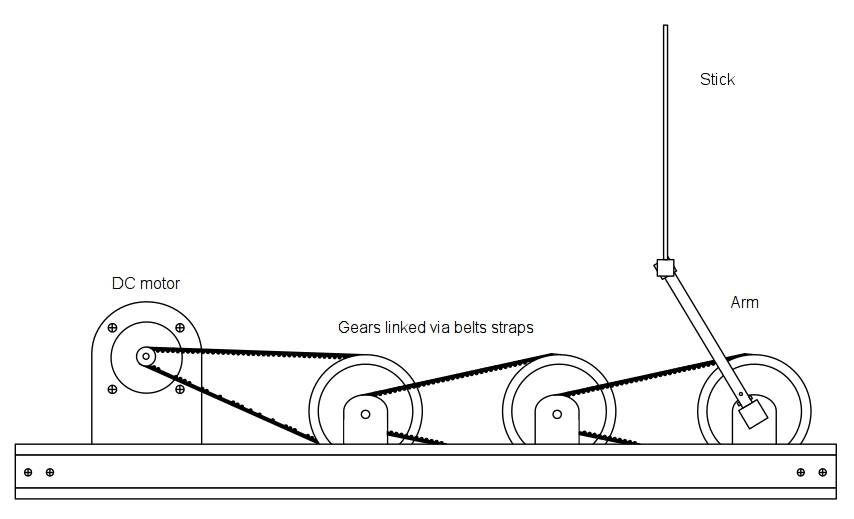
\includegraphics[width=0.7\linewidth]{figures/"Preanalysis&Requirement"/invertedPendulumDiagram}
	\caption{Diagram of the inverted pendulum setup\citep{web:BalancingStick2008}.} \label{fig:InvertedPendulum1}
\end{figure}


Construction and modeling of the rocket will be limited to a minor-scale rocket with a similarities to the design behind a full-scale rocket. The rocket will be designed around a solid propellant thruster, and will therefore not contain any liquid fuel. This is to limit the constraints from laws and keep the cost low. Further more weight and dimension limits is set before designing the rocket.
 
 
\textbf{Control delimitation:}
A choice is made that the starting point for controlling the stick is as illustrated cf. figure \ref{fig:InvertedPendulum1} in upwards vertical position. Therefore the controller will not be able to balance the stick, if its vertical balance limits is surpassed. The delimitation is made to simplify the controlling, and make it as similar as possible to controlling a rocket. 
 
 
\textbf{Test delimitation:}
Launching and flight of a rocket for testing a controller is a high cost procedure because of the chance of damaging the rocket and the cost of thrusters per launch. The testing of the rockets stabilization will be ground based test setup, where the controller can be tested without the risk of damaging the rocket. If, and only if the control system proves stable and safe, a launch and flight of the rocket will be conducted under circumstances fulfilling given laws.   
\bigbreak


The delimitation sets the boundaries for the project and describes which models is available. This gives possibility for describing and modeling of both the inverted pendulum and rocket, to examine if there is similarities behind controlling them. 